\documentclass[1p]{elsarticle_modified}
%\bibliographystyle{elsarticle-num}

%\usepackage[colorlinks]{hyperref}
%\usepackage{abbrmath_seonhwa} %\Abb, \Ascr, \Acal ,\Abf, \Afrak
\usepackage{amsfonts}
\usepackage{amssymb}
\usepackage{amsmath}
\usepackage{amsthm}
\usepackage{scalefnt}
\usepackage{amsbsy}
\usepackage{kotex}
\usepackage{caption}
\usepackage{subfig}
\usepackage{color}
\usepackage{graphicx}
\usepackage{xcolor} %% white, black, red, green, blue, cyan, magenta, yellow
\usepackage{float}
\usepackage{setspace}
\usepackage{hyperref}

\usepackage{tikz}
\usetikzlibrary{arrows}

\usepackage{multirow}
\usepackage{array} % fixed length table
\usepackage{hhline}

%%%%%%%%%%%%%%%%%%%%%
\makeatletter
\renewcommand*\env@matrix[1][\arraystretch]{%
	\edef\arraystretch{#1}%
	\hskip -\arraycolsep
	\let\@ifnextchar\new@ifnextchar
	\array{*\c@MaxMatrixCols c}}
\makeatother %https://tex.stackexchange.com/questions/14071/how-can-i-increase-the-line-spacing-in-a-matrix
%%%%%%%%%%%%%%%

\usepackage[normalem]{ulem}

\newcommand{\msout}[1]{\ifmmode\text{\sout{\ensuremath{#1}}}\else\sout{#1}\fi}
%SOURCE: \msout is \stkout macro in https://tex.stackexchange.com/questions/20609/strikeout-in-math-mode

\newcommand{\cancel}[1]{
	\ifmmode
	{\color{red}\msout{#1}}
	\else
	{\color{red}\sout{#1}}
	\fi
}

\newcommand{\add}[1]{
	{\color{blue}\uwave{#1}}
}

\newcommand{\replace}[2]{
	\ifmmode
	{\color{red}\msout{#1}}{\color{blue}\uwave{#2}}
	\else
	{\color{red}\sout{#1}}{\color{blue}\uwave{#2}}
	\fi
}

\newcommand{\Sol}{\mathcal{S}} %segment
\newcommand{\D}{D} %diagram
\newcommand{\A}{\mathcal{A}} %arc


%%%%%%%%%%%%%%%%%%%%%%%%%%%%%5 test

\def\sl{\operatorname{\textup{SL}}(2,\Cbb)}
\def\psl{\operatorname{\textup{PSL}}(2,\Cbb)}
\def\quan{\mkern 1mu \triangleright \mkern 1mu}

\theoremstyle{definition}
\newtheorem{thm}{Theorem}[section]
\newtheorem{prop}[thm]{Proposition}
\newtheorem{lem}[thm]{Lemma}
\newtheorem{ques}[thm]{Question}
\newtheorem{cor}[thm]{Corollary}
\newtheorem{defn}[thm]{Definition}
\newtheorem{exam}[thm]{Example}
\newtheorem{rmk}[thm]{Remark}
\newtheorem{alg}[thm]{Algorithm}

\newcommand{\I}{\sqrt{-1}}
\begin{document}

%\begin{frontmatter}
%
%\title{Boundary parabolic representations of knots up to 8 crossings}
%
%%% Group authors per affiliation:
%\author{Yunhi Cho} 
%\address{Department of Mathematics, University of Seoul, Seoul, Korea}
%\ead{yhcho@uos.ac.kr}
%
%
%\author{Seonhwa Kim} %\fnref{s_kim}}
%\address{Center for Geometry and Physics, Institute for Basic Science, Pohang, 37673, Korea}
%\ead{ryeona17@ibs.re.kr}
%
%\author{Hyuk Kim}
%\address{Department of Mathematical Sciences, Seoul National University, Seoul 08826, Korea}
%\ead{hyukkim@snu.ac.kr}
%
%\author{Seokbeom Yoon}
%\address{Department of Mathematical Sciences, Seoul National University, Seoul, 08826,  Korea}
%\ead{sbyoon15@snu.ac.kr}
%
%\begin{abstract}
%We find all boundary parabolic representation of knots up to 8 crossings.
%
%\end{abstract}
%\begin{keyword}
%    \MSC[2010] 57M25 
%\end{keyword}
%
%\end{frontmatter}

%\linenumbers
%\tableofcontents
%
\newcommand\colored[1]{\textcolor{white}{\rule[-0.35ex]{0.8em}{1.4ex}}\kern-0.8em\color{red} #1}%
%\newcommand\colored[1]{\textcolor{white}{ #1}\kern-2.17ex	\textcolor{white}{ #1}\kern-1.81ex	\textcolor{white}{ #1}\kern-2.15ex\color{red}#1	}

{\Large $\underline{12n_{0625}~(K12n_{0625})}$}

\setlength{\tabcolsep}{10pt}
\renewcommand{\arraystretch}{1.6}
\vspace{1cm}\begin{tabular}{m{100pt}>{\centering\arraybackslash}m{274pt}}
\multirow{5}{120pt}{
	\centering
	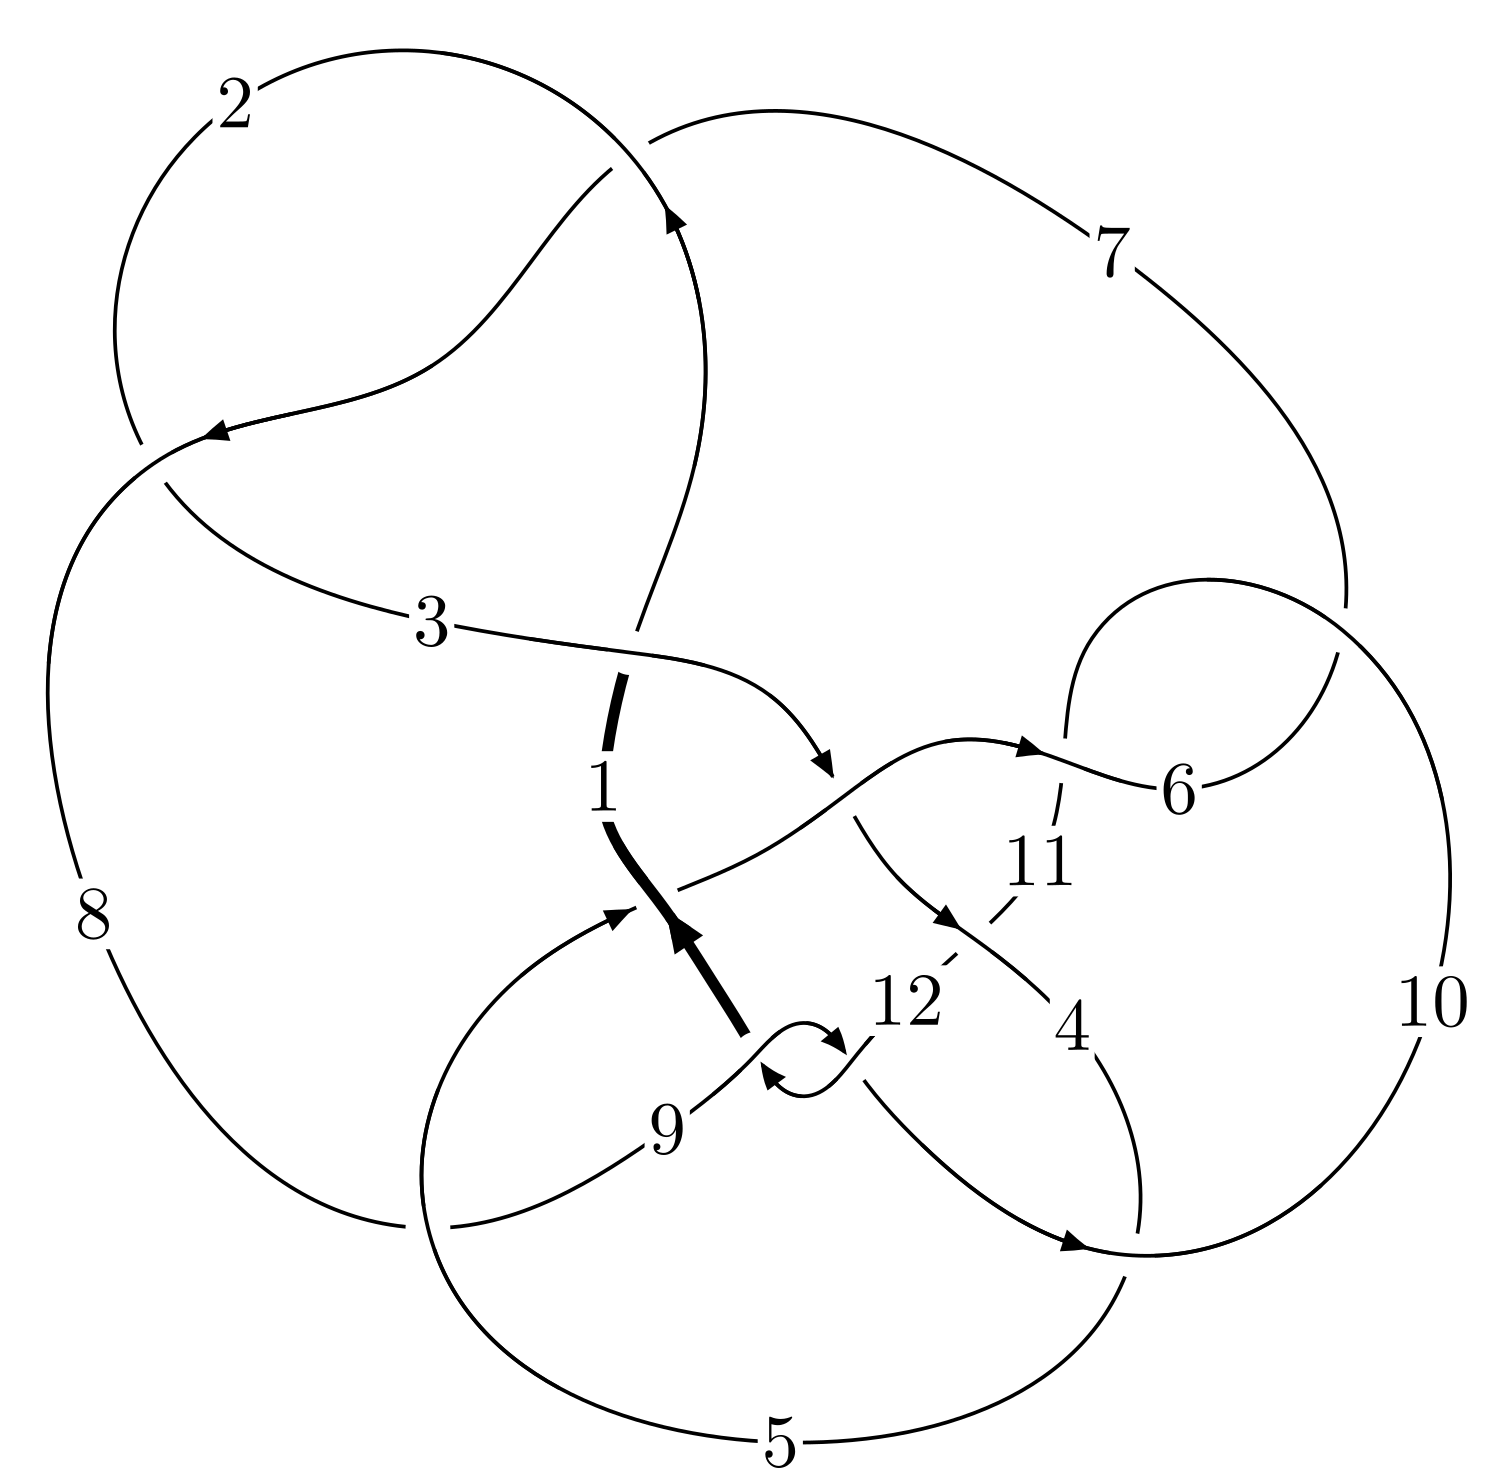
\includegraphics[width=112pt]{../../../GIT/diagram.site/Diagrams/png/2714_12n_0625.png}\\
\ \ \ A knot diagram\footnotemark}&
\allowdisplaybreaks
\textbf{Linearized knot diagam} \\
\cline{2-2}
 &
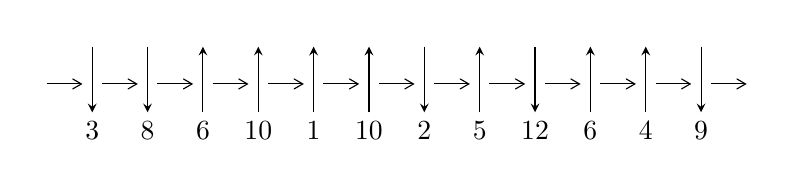
\begin{tikzpicture}[x=20pt, y=17pt]
	% nodes
	\node (C0) at (0, 0) {};
	\node (C1) at (1, 0) {};
	\node (C1U) at (1, +1) {};
	\node (C1D) at (1, -1) {3};

	\node (C2) at (2, 0) {};
	\node (C2U) at (2, +1) {};
	\node (C2D) at (2, -1) {8};

	\node (C3) at (3, 0) {};
	\node (C3U) at (3, +1) {};
	\node (C3D) at (3, -1) {6};

	\node (C4) at (4, 0) {};
	\node (C4U) at (4, +1) {};
	\node (C4D) at (4, -1) {10};

	\node (C5) at (5, 0) {};
	\node (C5U) at (5, +1) {};
	\node (C5D) at (5, -1) {1};

	\node (C6) at (6, 0) {};
	\node (C6U) at (6, +1) {};
	\node (C6D) at (6, -1) {10};

	\node (C7) at (7, 0) {};
	\node (C7U) at (7, +1) {};
	\node (C7D) at (7, -1) {2};

	\node (C8) at (8, 0) {};
	\node (C8U) at (8, +1) {};
	\node (C8D) at (8, -1) {5};

	\node (C9) at (9, 0) {};
	\node (C9U) at (9, +1) {};
	\node (C9D) at (9, -1) {12};

	\node (C10) at (10, 0) {};
	\node (C10U) at (10, +1) {};
	\node (C10D) at (10, -1) {6};

	\node (C11) at (11, 0) {};
	\node (C11U) at (11, +1) {};
	\node (C11D) at (11, -1) {4};

	\node (C12) at (12, 0) {};
	\node (C12U) at (12, +1) {};
	\node (C12D) at (12, -1) {9};
	\node (C13) at (13, 0) {};

	% arrows
	\draw[->,>={angle 60}]
	(C0) edge (C1) (C1) edge (C2) (C2) edge (C3) (C3) edge (C4) (C4) edge (C5) (C5) edge (C6) (C6) edge (C7) (C7) edge (C8) (C8) edge (C9) (C9) edge (C10) (C10) edge (C11) (C11) edge (C12) (C12) edge (C13) ;	\draw[->,>=stealth]
	(C1U) edge (C1D) (C2U) edge (C2D) (C3D) edge (C3U) (C4D) edge (C4U) (C5D) edge (C5U) (C6D) edge (C6U) (C7U) edge (C7D) (C8D) edge (C8U) (C9U) edge (C9D) (C10D) edge (C10U) (C11D) edge (C11U) (C12U) edge (C12D) ;
	\end{tikzpicture} \\
\hhline{~~} \\& 
\textbf{Solving Sequence} \\ \cline{2-2} 
 &
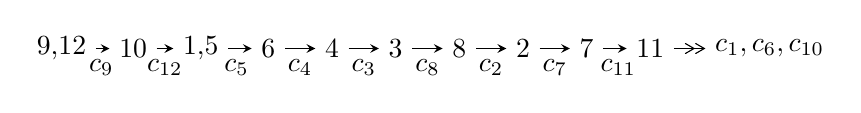
\begin{tikzpicture}[x=23pt, y=7pt]
	% node
	\node (A0) at (-1/8, 0) {9,12};
	\node (A1) at (1, 0) {10};
	\node (A2) at (33/16, 0) {1,5};
	\node (A3) at (25/8, 0) {6};
	\node (A4) at (33/8, 0) {4};
	\node (A5) at (41/8, 0) {3};
	\node (A6) at (49/8, 0) {8};
	\node (A7) at (57/8, 0) {2};
	\node (A8) at (65/8, 0) {7};
	\node (A9) at (73/8, 0) {11};
	\node (C1) at (1/2, -1) {$c_{9}$};
	\node (C2) at (3/2, -1) {$c_{12}$};
	\node (C3) at (21/8, -1) {$c_{5}$};
	\node (C4) at (29/8, -1) {$c_{4}$};
	\node (C5) at (37/8, -1) {$c_{3}$};
	\node (C6) at (45/8, -1) {$c_{8}$};
	\node (C7) at (53/8, -1) {$c_{2}$};
	\node (C8) at (61/8, -1) {$c_{7}$};
	\node (C9) at (69/8, -1) {$c_{11}$};
	\node (A10) at (11, 0) {$c_{1},c_{6},c_{10}$};

	% edge
	\draw[->,>=stealth]	
	(A0) edge (A1) (A1) edge (A2) (A2) edge (A3) (A3) edge (A4) (A4) edge (A5) (A5) edge (A6) (A6) edge (A7) (A7) edge (A8) (A8) edge (A9) ;
	\draw[->>,>={angle 60}]	
	(A9) edge (A10);
\end{tikzpicture} \\ 

\end{tabular} \\

\footnotetext{
The image of knot diagram is generated by the software ``\textbf{Draw programme}" developed by Andrew Bartholomew(\url{http://www.layer8.co.uk/maths/draw/index.htm\#Running-draw}), where we modified some parts for our purpose(\url{https://github.com/CATsTAILs/LinksPainter}).
}\phantom \\ \newline 
\centering \textbf{Ideals for irreducible components\footnotemark of $X_{\text{par}}$} 
 
\begin{align*}
I^u_{1}&=\langle 
-97 u^{34}-1164 u^{33}+\cdots+4 b-1732,\;-239 u^{34}-2674 u^{33}+\cdots+8 a-4156,\\
\phantom{I^u_{1}}&\phantom{= \langle  }u^{35}+12 u^{34}+\cdots+140 u+8\rangle \\
I^u_{2}&=\langle 
-3 u^{24}+20 u^{23}+\cdots+b-14,\;14 u^{25}-83 u^{24}+\cdots+5 a+15,\;u^{26}-7 u^{25}+\cdots-15 u+5\rangle \\
I^u_{3}&=\langle 
-38441817751 a^5 u^5-19856412660 u^5 a^4+\cdots-2635825958 a-179169756,\\
\phantom{I^u_{3}}&\phantom{= \langle  }4 u^5 a^4+u^5 a^3+\cdots+90 a-272,\;u^6- u^5+3 u^4-2 u^3+2 u^2- u-1\rangle \\
\\
\end{align*}
\raggedright * 3 irreducible components of $\dim_{\mathbb{C}}=0$, with total 97 representations.\\
\footnotetext{All coefficients of polynomials are rational numbers. But the coefficients are sometimes approximated in decimal forms when there is not enough margin.}
\newpage
\renewcommand{\arraystretch}{1}
\centering \section*{I. $I^u_{1}= \langle -97 u^{34}-1164 u^{33}+\cdots+4 b-1732,\;-239 u^{34}-2674 u^{33}+\cdots+8 a-4156,\;u^{35}+12 u^{34}+\cdots+140 u+8 \rangle$}
\flushleft \textbf{(i) Arc colorings}\\
\begin{tabular}{m{7pt} m{180pt} m{7pt} m{180pt} }
\flushright $a_{9}=$&$\begin{pmatrix}1\\0\end{pmatrix}$ \\
\flushright $a_{12}=$&$\begin{pmatrix}0\\u\end{pmatrix}$ \\
\flushright $a_{10}=$&$\begin{pmatrix}1\\u^2\end{pmatrix}$ \\
\flushright $a_{1}=$&$\begin{pmatrix}- u\\u\end{pmatrix}$ \\
\flushright $a_{5}=$&$\begin{pmatrix}29.8750 u^{34}+334.250 u^{33}+\cdots+7861.75 u+519.500\\\frac{97}{4} u^{34}+291 u^{33}+\cdots+6625 u+433\end{pmatrix}$ \\
\flushright $a_{6}=$&$\begin{pmatrix}29.8750 u^{34}+344.250 u^{33}+\cdots+10823.8 u+713.500\\\frac{97}{4} u^{34}+281 u^{33}+\cdots+3663 u+239\end{pmatrix}$ \\
\flushright $a_{4}=$&$\begin{pmatrix}15.6250 u^{34}+177.250 u^{33}+\cdots+4392.75 u+280.500\\\frac{85}{4} u^{34}+243 u^{33}+\cdots+4779 u+321\end{pmatrix}$ \\
\flushright $a_{3}=$&$\begin{pmatrix}7.37500 u^{34}+71.2500 u^{33}+\cdots-4744.25 u-354.500\\\frac{21}{4} u^{34}+75 u^{33}+\cdots+4263 u+263\end{pmatrix}$ \\
\flushright $a_{8}=$&$\begin{pmatrix}-\frac{33}{8} u^{34}-\frac{191}{4} u^{33}+\cdots-\frac{3645}{4} u-56\\-\frac{17}{4} u^{34}-\frac{97}{2} u^{33}+\cdots-\frac{2097}{2} u-67\end{pmatrix}$ \\
\flushright $a_{2}=$&$\begin{pmatrix}-\frac{125}{8} u^{34}-\frac{727}{4} u^{33}+\cdots-\frac{28857}{4} u-491\\-\frac{15}{4} u^{34}-\frac{93}{2} u^{33}+\cdots+\frac{313}{2} u+7\end{pmatrix}$ \\
\flushright $a_{7}=$&$\begin{pmatrix}-40.1250 u^{34}-460.250 u^{33}+\cdots-12730.8 u-838.500\\-\frac{89}{4} u^{34}-265 u^{33}+\cdots-4561 u-295\end{pmatrix}$ \\
\flushright $a_{11}=$&$\begin{pmatrix}\frac{5}{8} u^{34}+\frac{27}{4} u^{33}+\cdots+\frac{233}{4} u+4\\-\frac{1}{4} u^{34}-\frac{5}{2} u^{33}+\cdots+\frac{33}{2} u+1\end{pmatrix}$\\&\end{tabular}
\flushleft \textbf{(ii) Obstruction class $= -1$}\\~\\
\flushleft \textbf{(iii) Cusp Shapes $= - u^{34}-40 u^{33}+\cdots-3016 u-210$}\\~\\
\newpage\renewcommand{\arraystretch}{1}
\flushleft \textbf{(iv) u-Polynomials at the component}\newline \\
\begin{tabular}{m{50pt}|m{274pt}}
Crossings & \hspace{64pt}u-Polynomials at each crossing \\
\hline $$\begin{aligned}c_{1}\end{aligned}$$&$\begin{aligned}
&u^{35}+17 u^{34}+\cdots-3072 u+4096
\end{aligned}$\\
\hline $$\begin{aligned}c_{2},c_{7}\end{aligned}$$&$\begin{aligned}
&u^{35}-13 u^{34}+\cdots-544 u+64
\end{aligned}$\\
\hline $$\begin{aligned}c_{3}\end{aligned}$$&$\begin{aligned}
&u^{35}+19 u^{34}+\cdots+20188 u+1960
\end{aligned}$\\
\hline $$\begin{aligned}c_{4}\end{aligned}$$&$\begin{aligned}
&u^{35}-19 u^{33}+\cdots+270 u-193
\end{aligned}$\\
\hline $$\begin{aligned}c_{5},c_{8}\end{aligned}$$&$\begin{aligned}
&u^{35}-12 u^{33}+\cdots+10 u-1
\end{aligned}$\\
\hline $$\begin{aligned}c_{6},c_{10},c_{11}\end{aligned}$$&$\begin{aligned}
&u^{35}- u^{34}+\cdots-16 u^2+1
\end{aligned}$\\
\hline $$\begin{aligned}c_{9},c_{12}\end{aligned}$$&$\begin{aligned}
&u^{35}-12 u^{34}+\cdots+140 u-8
\end{aligned}$\\
\hline
\end{tabular}\\~\\
\newpage\renewcommand{\arraystretch}{1}
\flushleft \textbf{(v) Riley Polynomials at the component}\newline \\
\begin{tabular}{m{50pt}|m{274pt}}
Crossings & \hspace{64pt}Riley Polynomials at each crossing \\
\hline $$\begin{aligned}c_{1}\end{aligned}$$&$\begin{aligned}
&y^{35}+3 y^{34}+\cdots-250609664 y-16777216
\end{aligned}$\\
\hline $$\begin{aligned}c_{2},c_{7}\end{aligned}$$&$\begin{aligned}
&y^{35}-17 y^{34}+\cdots-3072 y-4096
\end{aligned}$\\
\hline $$\begin{aligned}c_{3}\end{aligned}$$&$\begin{aligned}
&y^{35}-45 y^{34}+\cdots+57342544 y-3841600
\end{aligned}$\\
\hline $$\begin{aligned}c_{4}\end{aligned}$$&$\begin{aligned}
&y^{35}-38 y^{34}+\cdots-208108 y-37249
\end{aligned}$\\
\hline $$\begin{aligned}c_{5},c_{8}\end{aligned}$$&$\begin{aligned}
&y^{35}-24 y^{34}+\cdots+34 y-1
\end{aligned}$\\
\hline $$\begin{aligned}c_{6},c_{10},c_{11}\end{aligned}$$&$\begin{aligned}
&y^{35}-55 y^{34}+\cdots+32 y-1
\end{aligned}$\\
\hline $$\begin{aligned}c_{9},c_{12}\end{aligned}$$&$\begin{aligned}
&y^{35}+24 y^{34}+\cdots+912 y-64
\end{aligned}$\\
\hline
\end{tabular}\\~\\
\newpage\flushleft \textbf{(vi) Complex Volumes and Cusp Shapes}
$$\begin{array}{c|c|c}  
\text{Solutions to }I^u_{1}& \I (\text{vol} + \sqrt{-1}CS) & \text{Cusp shape}\\
 \hline 
\begin{aligned}
u &= -1.099980 + 0.143930 I \\
a &= \phantom{-}0.230693 - 0.044757 I \\
b &= -1.19145 - 0.89068 I\end{aligned}
 & \phantom{-}8.07701 + 10.47920 I & \phantom{-0.000000 } 0 \\ \hline\begin{aligned}
u &= -1.099980 - 0.143930 I \\
a &= \phantom{-}0.230693 + 0.044757 I \\
b &= -1.19145 + 0.89068 I\end{aligned}
 & \phantom{-}8.07701 - 10.47920 I & \phantom{-0.000000 } 0 \\ \hline\begin{aligned}
u &= -0.176786 + 1.110160 I \\
a &= -1.50400 - 0.06191 I \\
b &= \phantom{-}0.819836 + 0.909342 I\end{aligned}
 & -0.154709 + 0.705431 I & \phantom{-0.000000 } 0 \\ \hline\begin{aligned}
u &= -0.176786 - 1.110160 I \\
a &= -1.50400 + 0.06191 I \\
b &= \phantom{-}0.819836 - 0.909342 I\end{aligned}
 & -0.154709 - 0.705431 I & \phantom{-0.000000 } 0 \\ \hline\begin{aligned}
u &= -1.148150 + 0.105837 I \\
a &= -0.218382 + 0.022702 I \\
b &= \phantom{-}1.266830 + 0.573062 I\end{aligned}
 & \phantom{-}9.98543 + 3.73790 I & \phantom{-0.000000 } 0 \\ \hline\begin{aligned}
u &= -1.148150 - 0.105837 I \\
a &= -0.218382 - 0.022702 I \\
b &= \phantom{-}1.266830 - 0.573062 I\end{aligned}
 & \phantom{-}9.98543 - 3.73790 I & \phantom{-0.000000 } 0 \\ \hline\begin{aligned}
u &= -0.156742 + 1.187670 I \\
a &= \phantom{-}1.74113 - 0.29318 I \\
b &= -1.21323 - 0.79801 I\end{aligned}
 & \phantom{-}4.43767 + 2.72692 I & \phantom{-0.000000 } 0 \\ \hline\begin{aligned}
u &= -0.156742 - 1.187670 I \\
a &= \phantom{-}1.74113 + 0.29318 I \\
b &= -1.21323 + 0.79801 I\end{aligned}
 & \phantom{-}4.43767 - 2.72692 I & \phantom{-0.000000 } 0 \\ \hline\begin{aligned}
u &= -0.080256 + 1.203320 I \\
a &= \phantom{-}1.32268 - 0.52185 I \\
b &= -1.066100 - 0.381230 I\end{aligned}
 & \phantom{-}5.03943 + 0.52910 I & \phantom{-0.000000 } 0 \\ \hline\begin{aligned}
u &= -0.080256 - 1.203320 I \\
a &= \phantom{-}1.32268 + 0.52185 I \\
b &= -1.066100 + 0.381230 I\end{aligned}
 & \phantom{-}5.03943 - 0.52910 I & \phantom{-0.000000 } 0\\
 \hline 
 \end{array}$$\newpage$$\begin{array}{c|c|c}  
\text{Solutions to }I^u_{1}& \I (\text{vol} + \sqrt{-1}CS) & \text{Cusp shape}\\
 \hline 
\begin{aligned}
u &= -0.180648 + 1.194610 I \\
a &= -1.91566 + 0.20321 I \\
b &= \phantom{-}1.28335 + 0.96670 I\end{aligned}
 & \phantom{-}2.44479 + 7.71496 I & \phantom{-0.000000 } 0 \\ \hline\begin{aligned}
u &= -0.180648 - 1.194610 I \\
a &= -1.91566 - 0.20321 I \\
b &= \phantom{-}1.28335 - 0.96670 I\end{aligned}
 & \phantom{-}2.44479 - 7.71496 I & \phantom{-0.000000 } 0 \\ \hline\begin{aligned}
u &= -0.027618 + 1.240640 I \\
a &= -1.043420 + 0.623249 I \\
b &= \phantom{-}0.946278 + 0.141646 I\end{aligned}
 & \phantom{-}3.62037 - 4.19606 I & \phantom{-0.000000 } 0 \\ \hline\begin{aligned}
u &= -0.027618 - 1.240640 I \\
a &= -1.043420 - 0.623249 I \\
b &= \phantom{-}0.946278 - 0.141646 I\end{aligned}
 & \phantom{-}3.62037 + 4.19606 I & \phantom{-0.000000 } 0 \\ \hline\begin{aligned}
u &= \phantom{-}0.393608 + 0.616666 I \\
a &= -0.541312 - 0.331797 I \\
b &= \phantom{-}0.128387 + 0.276430 I\end{aligned}
 & \phantom{-}0.073195 - 1.283670 I & \phantom{-}0.53283 + 5.86961 I \\ \hline\begin{aligned}
u &= \phantom{-}0.393608 - 0.616666 I \\
a &= -0.541312 + 0.331797 I \\
b &= \phantom{-}0.128387 - 0.276430 I\end{aligned}
 & \phantom{-}0.073195 + 1.283670 I & \phantom{-}0.53283 - 5.86961 I \\ \hline\begin{aligned}
u &= -1.33744\phantom{ +0.000000I} \\
a &= \phantom{-}0.212540\phantom{ +0.000000I} \\
b &= -0.842391\phantom{ +0.000000I}\end{aligned}
 & \phantom{-}1.80982\phantom{ +0.000000I} & \phantom{-0.000000 } 0 \\ \hline\begin{aligned}
u &= -0.382949 + 0.400086 I \\
a &= \phantom{-}1.077350 + 0.149282 I \\
b &= \phantom{-}0.262290 - 0.775953 I\end{aligned}
 & -2.26874 + 1.67313 I & \phantom{-}1.23489 - 1.13105 I \\ \hline\begin{aligned}
u &= -0.382949 - 0.400086 I \\
a &= \phantom{-}1.077350 - 0.149282 I \\
b &= \phantom{-}0.262290 + 0.775953 I\end{aligned}
 & -2.26874 - 1.67313 I & \phantom{-}1.23489 + 1.13105 I \\ \hline\begin{aligned}
u &= -0.48137 + 1.41511 I \\
a &= \phantom{-}1.87041 - 0.11510 I \\
b &= -1.51506 - 1.07641 I\end{aligned}
 & \phantom{-}12.9957 + 16.0498 I & \phantom{-0.000000 } 0\\
 \hline 
 \end{array}$$\newpage$$\begin{array}{c|c|c}  
\text{Solutions to }I^u_{1}& \I (\text{vol} + \sqrt{-1}CS) & \text{Cusp shape}\\
 \hline 
\begin{aligned}
u &= -0.48137 - 1.41511 I \\
a &= \phantom{-}1.87041 + 0.11510 I \\
b &= -1.51506 + 1.07641 I\end{aligned}
 & \phantom{-}12.9957 - 16.0498 I & \phantom{-0.000000 } 0 \\ \hline\begin{aligned}
u &= -0.50191 + 1.42077 I \\
a &= -1.72676 + 0.32922 I \\
b &= \phantom{-}1.55368 + 0.82547 I\end{aligned}
 & \phantom{-}14.8329 + 9.5367 I & \phantom{-0.000000 } 0 \\ \hline\begin{aligned}
u &= -0.50191 - 1.42077 I \\
a &= -1.72676 - 0.32922 I \\
b &= \phantom{-}1.55368 - 0.82547 I\end{aligned}
 & \phantom{-}14.8329 - 9.5367 I & \phantom{-0.000000 } 0 \\ \hline\begin{aligned}
u &= \phantom{-}1.08815 + 1.05620 I \\
a &= \phantom{-}0.209018 + 0.062343 I \\
b &= -0.1172880 - 0.0788852 I\end{aligned}
 & -5.12951 - 4.01720 I & \phantom{-0.000000 } 0 \\ \hline\begin{aligned}
u &= \phantom{-}1.08815 - 1.05620 I \\
a &= \phantom{-}0.209018 - 0.062343 I \\
b &= -0.1172880 + 0.0788852 I\end{aligned}
 & -5.12951 + 4.01720 I & \phantom{-0.000000 } 0 \\ \hline\begin{aligned}
u &= -0.67357 + 1.36899 I \\
a &= \phantom{-}0.486870 - 0.931148 I \\
b &= -1.050210 + 0.441181 I\end{aligned}
 & \phantom{-}11.70210 - 4.12793 I & \phantom{-0.000000 } 0 \\ \hline\begin{aligned}
u &= -0.67357 - 1.36899 I \\
a &= \phantom{-}0.486870 + 0.931148 I \\
b &= -1.050210 - 0.441181 I\end{aligned}
 & \phantom{-}11.70210 + 4.12793 I & \phantom{-0.000000 } 0 \\ \hline\begin{aligned}
u &= -0.61726 + 1.41428 I \\
a &= -0.858106 + 0.838071 I \\
b &= \phantom{-}1.257250 - 0.123309 I\end{aligned}
 & \phantom{-}14.0234 + 2.6592 I & \phantom{-0.000000 } 0 \\ \hline\begin{aligned}
u &= -0.61726 - 1.41428 I \\
a &= -0.858106 - 0.838071 I \\
b &= \phantom{-}1.257250 + 0.123309 I\end{aligned}
 & \phantom{-}14.0234 - 2.6592 I & \phantom{-0.000000 } 0 \\ \hline\begin{aligned}
u &= -0.412094 + 0.136239 I \\
a &= \phantom{-}1.48498 - 0.11016 I \\
b &= \phantom{-}0.870960 - 0.623172 I\end{aligned}
 & -0.69807 - 5.41461 I & \phantom{-}4.99900 + 9.86847 I\\
 \hline 
 \end{array}$$\newpage$$\begin{array}{c|c|c}  
\text{Solutions to }I^u_{1}& \I (\text{vol} + \sqrt{-1}CS) & \text{Cusp shape}\\
 \hline 
\begin{aligned}
u &= -0.412094 - 0.136239 I \\
a &= \phantom{-}1.48498 + 0.11016 I \\
b &= \phantom{-}0.870960 + 0.623172 I\end{aligned}
 & -0.69807 + 5.41461 I & \phantom{-}4.99900 - 9.86847 I \\ \hline\begin{aligned}
u &= -0.53677 + 1.49180 I \\
a &= \phantom{-}1.111360 - 0.251453 I \\
b &= -1.054110 - 0.475748 I\end{aligned}
 & \phantom{-}6.80622 + 6.65686 I & \phantom{-0.000000 } 0 \\ \hline\begin{aligned}
u &= -0.53677 - 1.49180 I \\
a &= \phantom{-}1.111360 + 0.251453 I \\
b &= -1.054110 + 0.475748 I\end{aligned}
 & \phantom{-}6.80622 - 6.65686 I & \phantom{-0.000000 } 0 \\ \hline\begin{aligned}
u &= -0.336936 + 0.095632 I \\
a &= -1.58311 - 0.02068 I \\
b &= -0.760213 + 0.327462 I\end{aligned}
 & \phantom{-}1.31189 - 0.75210 I & \phantom{-}6.86398 + 3.34403 I \\ \hline\begin{aligned}
u &= -0.336936 - 0.095632 I \\
a &= -1.58311 + 0.02068 I \\
b &= -0.760213 - 0.327462 I\end{aligned}
 & \phantom{-}1.31189 + 0.75210 I & \phantom{-}6.86398 - 3.34403 I\\
 \hline 
 \end{array}$$\newpage\newpage\renewcommand{\arraystretch}{1}
\centering \section*{II. $I^u_{2}= \langle -3 u^{24}+20 u^{23}+\cdots+b-14,\;14 u^{25}-83 u^{24}+\cdots+5 a+15,\;u^{26}-7 u^{25}+\cdots-15 u+5 \rangle$}
\flushleft \textbf{(i) Arc colorings}\\
\begin{tabular}{m{7pt} m{180pt} m{7pt} m{180pt} }
\flushright $a_{9}=$&$\begin{pmatrix}1\\0\end{pmatrix}$ \\
\flushright $a_{12}=$&$\begin{pmatrix}0\\u\end{pmatrix}$ \\
\flushright $a_{10}=$&$\begin{pmatrix}1\\u^2\end{pmatrix}$ \\
\flushright $a_{1}=$&$\begin{pmatrix}- u\\u\end{pmatrix}$ \\
\flushright $a_{5}=$&$\begin{pmatrix}-\frac{14}{5} u^{25}+\frac{83}{5} u^{24}+\cdots+\frac{1}{5} u-3\\3 u^{24}-20 u^{23}+\cdots-31 u+14\end{pmatrix}$ \\
\flushright $a_{6}=$&$\begin{pmatrix}\frac{1}{5} u^{25}-\frac{17}{5} u^{24}+\cdots+\frac{71}{5} u-3\\-3 u^{25}+23 u^{24}+\cdots-45 u+14\end{pmatrix}$ \\
\flushright $a_{4}=$&$\begin{pmatrix}-\frac{4}{5} u^{25}+\frac{28}{5} u^{24}+\cdots+\frac{1}{5} u-2\\-2 u^{22}+11 u^{21}+\cdots+4 u-1\end{pmatrix}$ \\
\flushright $a_{3}=$&$\begin{pmatrix}-\frac{21}{5} u^{25}+\frac{152}{5} u^{24}+\cdots-\frac{181}{5} u+5\\8 u^{25}-54 u^{24}+\cdots+50 u-9\end{pmatrix}$ \\
\flushright $a_{8}=$&$\begin{pmatrix}\frac{9}{5} u^{25}-\frac{53}{5} u^{24}+\cdots-\frac{11}{5} u+5\\u^{25}-8 u^{24}+\cdots+32 u-14\end{pmatrix}$ \\
\flushright $a_{2}=$&$\begin{pmatrix}-\frac{9}{5} u^{25}+\frac{93}{5} u^{24}+\cdots-\frac{259}{5} u+17\\6 u^{25}-47 u^{24}+\cdots+88 u-26\end{pmatrix}$ \\
\flushright $a_{7}=$&$\begin{pmatrix}\frac{1}{5} u^{25}-\frac{7}{5} u^{24}+\cdots+\frac{1}{5} u+1\\2 u^{24}-13 u^{23}+\cdots-15 u+4\end{pmatrix}$ \\
\flushright $a_{11}=$&$\begin{pmatrix}\frac{6}{5} u^{25}-\frac{42}{5} u^{24}+\cdots+\frac{11}{5} u-1\\- u^{25}+6 u^{24}+\cdots+11 u-6\end{pmatrix}$\\&\end{tabular}
\flushleft \textbf{(ii) Obstruction class $= 1$}\\~\\
\flushleft \textbf{(iii) Cusp Shapes $= 2 u^{25}+9 u^{24}-77 u^{23}+407 u^{22}-1373 u^{21}+3767 u^{20}-8362 u^{19}+15938 u^{18}-25873 u^{17}+36425 u^{16}-43673 u^{15}+43799 u^{14}-33927 u^{13}+14898 u^{12}+8887 u^{11}-30580 u^{10}+44036 u^9-46418 u^8+39264 u^7-27167 u^6+15123 u^5-6437 u^4+1785 u^3-99 u^2-150 u+45$}\\~\\
\newpage\renewcommand{\arraystretch}{1}
\flushleft \textbf{(iv) u-Polynomials at the component}\newline \\
\begin{tabular}{m{50pt}|m{274pt}}
Crossings & \hspace{64pt}u-Polynomials at each crossing \\
\hline $$\begin{aligned}c_{1}\end{aligned}$$&$\begin{aligned}
&u^{26}-16 u^{25}+\cdots-115 u+9
\end{aligned}$\\
\hline $$\begin{aligned}c_{2}\end{aligned}$$&$\begin{aligned}
&u^{26}-8 u^{24}+\cdots+5 u+3
\end{aligned}$\\
\hline $$\begin{aligned}c_{3}\end{aligned}$$&$\begin{aligned}
&u^{26}+22 u^{25}+\cdots+3110 u+473
\end{aligned}$\\
\hline $$\begin{aligned}c_{4}\end{aligned}$$&$\begin{aligned}
&u^{26}-9 u^{24}+\cdots- u-3
\end{aligned}$\\
\hline $$\begin{aligned}c_{5},c_{8}\end{aligned}$$&$\begin{aligned}
&u^{26}+2 u^{24}+\cdots-7 u-1
\end{aligned}$\\
\hline $$\begin{aligned}c_{6},c_{11}\end{aligned}$$&$\begin{aligned}
&u^{26}- u^{25}+\cdots+u-1
\end{aligned}$\\
\hline $$\begin{aligned}c_{7}\end{aligned}$$&$\begin{aligned}
&u^{26}-8 u^{24}+\cdots-5 u+3
\end{aligned}$\\
\hline $$\begin{aligned}c_{9}\end{aligned}$$&$\begin{aligned}
&u^{26}-7 u^{25}+\cdots-15 u+5
\end{aligned}$\\
\hline $$\begin{aligned}c_{10}\end{aligned}$$&$\begin{aligned}
&u^{26}+u^{25}+\cdots- u-1
\end{aligned}$\\
\hline $$\begin{aligned}c_{12}\end{aligned}$$&$\begin{aligned}
&u^{26}+7 u^{25}+\cdots+15 u+5
\end{aligned}$\\
\hline
\end{tabular}\\~\\
\newpage\renewcommand{\arraystretch}{1}
\flushleft \textbf{(v) Riley Polynomials at the component}\newline \\
\begin{tabular}{m{50pt}|m{274pt}}
Crossings & \hspace{64pt}Riley Polynomials at each crossing \\
\hline $$\begin{aligned}c_{1}\end{aligned}$$&$\begin{aligned}
&y^{26}-4 y^{24}+\cdots-211 y+81
\end{aligned}$\\
\hline $$\begin{aligned}c_{2},c_{7}\end{aligned}$$&$\begin{aligned}
&y^{26}-16 y^{25}+\cdots-115 y+9
\end{aligned}$\\
\hline $$\begin{aligned}c_{3}\end{aligned}$$&$\begin{aligned}
&y^{26}-34 y^{25}+\cdots-2510880 y+223729
\end{aligned}$\\
\hline $$\begin{aligned}c_{4}\end{aligned}$$&$\begin{aligned}
&y^{26}-18 y^{25}+\cdots+47 y+9
\end{aligned}$\\
\hline $$\begin{aligned}c_{5},c_{8}\end{aligned}$$&$\begin{aligned}
&y^{26}+4 y^{25}+\cdots-27 y+1
\end{aligned}$\\
\hline $$\begin{aligned}c_{6},c_{10},c_{11}\end{aligned}$$&$\begin{aligned}
&y^{26}-19 y^{25}+\cdots+15 y+1
\end{aligned}$\\
\hline $$\begin{aligned}c_{9},c_{12}\end{aligned}$$&$\begin{aligned}
&y^{26}+19 y^{25}+\cdots-365 y+25
\end{aligned}$\\
\hline
\end{tabular}\\~\\
\newpage\flushleft \textbf{(vi) Complex Volumes and Cusp Shapes}
$$\begin{array}{c|c|c}  
\text{Solutions to }I^u_{2}& \I (\text{vol} + \sqrt{-1}CS) & \text{Cusp shape}\\
 \hline 
\begin{aligned}
u &= -0.994612\phantom{ +0.000000I} \\
a &= \phantom{-}0.638284\phantom{ +0.000000I} \\
b &= -0.318280\phantom{ +0.000000I}\end{aligned}
 & \phantom{-}0.856397\phantom{ +0.000000I} & -2.32000\phantom{ +0.000000I} \\ \hline\begin{aligned}
u &= -0.212241 + 1.020190 I \\
a &= \phantom{-}1.23563 - 1.37216 I \\
b &= -0.081295 + 1.211700 I\end{aligned}
 & \phantom{-}9.42472 - 2.04416 I & \phantom{-}6.12450 + 2.23947 I \\ \hline\begin{aligned}
u &= -0.212241 - 1.020190 I \\
a &= \phantom{-}1.23563 + 1.37216 I \\
b &= -0.081295 - 1.211700 I\end{aligned}
 & \phantom{-}9.42472 + 2.04416 I & \phantom{-}6.12450 - 2.23947 I \\ \hline\begin{aligned}
u &= \phantom{-}0.690336 + 0.610624 I \\
a &= \phantom{-}0.076479 - 0.614284 I \\
b &= \phantom{-}0.774243 + 0.308106 I\end{aligned}
 & \phantom{-}1.035900 - 0.601010 I & \phantom{-}6.74042 + 0.76556 I \\ \hline\begin{aligned}
u &= \phantom{-}0.690336 - 0.610624 I \\
a &= \phantom{-}0.076479 + 0.614284 I \\
b &= \phantom{-}0.774243 - 0.308106 I\end{aligned}
 & \phantom{-}1.035900 + 0.601010 I & \phantom{-}6.74042 - 0.76556 I \\ \hline\begin{aligned}
u &= -0.149267 + 1.091680 I \\
a &= -1.79375 + 0.98935 I \\
b &= \phantom{-}0.54342 - 1.31617 I\end{aligned}
 & \phantom{-}9.80770 + 3.58067 I & \phantom{-}6.57697 - 2.52937 I \\ \hline\begin{aligned}
u &= -0.149267 - 1.091680 I \\
a &= -1.79375 - 0.98935 I \\
b &= \phantom{-}0.54342 + 1.31617 I\end{aligned}
 & \phantom{-}9.80770 - 3.58067 I & \phantom{-}6.57697 + 2.52937 I \\ \hline\begin{aligned}
u &= \phantom{-}0.389539 + 1.134620 I \\
a &= -1.302210 - 0.416528 I \\
b &= \phantom{-}1.108030 - 0.626702 I\end{aligned}
 & \phantom{-}2.91227 - 3.60504 I & \phantom{-}3.99685 + 3.76042 I \\ \hline\begin{aligned}
u &= \phantom{-}0.389539 - 1.134620 I \\
a &= -1.302210 + 0.416528 I \\
b &= \phantom{-}1.108030 + 0.626702 I\end{aligned}
 & \phantom{-}2.91227 + 3.60504 I & \phantom{-}3.99685 - 3.76042 I \\ \hline\begin{aligned}
u &= \phantom{-}0.797638 + 0.055469 I \\
a &= -0.141851 - 0.260115 I \\
b &= -0.182422 - 1.114170 I\end{aligned}
 & -3.82284 - 1.29938 I & -2.97334 + 4.45756 I\\
 \hline 
 \end{array}$$\newpage$$\begin{array}{c|c|c}  
\text{Solutions to }I^u_{2}& \I (\text{vol} + \sqrt{-1}CS) & \text{Cusp shape}\\
 \hline 
\begin{aligned}
u &= \phantom{-}0.797638 - 0.055469 I \\
a &= -0.141851 + 0.260115 I \\
b &= -0.182422 + 1.114170 I\end{aligned}
 & -3.82284 + 1.29938 I & -2.97334 - 4.45756 I \\ \hline\begin{aligned}
u &= \phantom{-}0.332677 + 1.187440 I \\
a &= \phantom{-}1.67027 + 0.23671 I \\
b &= -1.22101 + 0.91742 I\end{aligned}
 & \phantom{-}1.60214 - 8.49569 I & \phantom{-}1.29011 + 9.18149 I \\ \hline\begin{aligned}
u &= \phantom{-}0.332677 - 1.187440 I \\
a &= \phantom{-}1.67027 - 0.23671 I \\
b &= -1.22101 - 0.91742 I\end{aligned}
 & \phantom{-}1.60214 + 8.49569 I & \phantom{-}1.29011 - 9.18149 I \\ \hline\begin{aligned}
u &= \phantom{-}0.663432 + 0.362819 I \\
a &= -0.524336 + 0.422708 I \\
b &= -0.822418 - 0.618568 I\end{aligned}
 & -1.08880 + 4.74486 I & -0.32078 - 1.84995 I \\ \hline\begin{aligned}
u &= \phantom{-}0.663432 - 0.362819 I \\
a &= -0.524336 - 0.422708 I \\
b &= -0.822418 + 0.618568 I\end{aligned}
 & -1.08880 - 4.74486 I & -0.32078 + 1.84995 I \\ \hline\begin{aligned}
u &= -0.084221 + 1.248750 I \\
a &= -1.63024 - 0.11402 I \\
b &= \phantom{-}1.036010 - 0.675543 I\end{aligned}
 & \phantom{-}7.45067 + 1.13341 I & \phantom{-}10.54209 + 2.52582 I \\ \hline\begin{aligned}
u &= -0.084221 - 1.248750 I \\
a &= -1.63024 + 0.11402 I \\
b &= \phantom{-}1.036010 + 0.675543 I\end{aligned}
 & \phantom{-}7.45067 - 1.13341 I & \phantom{-}10.54209 - 2.52582 I \\ \hline\begin{aligned}
u &= \phantom{-}0.352829 + 1.277260 I \\
a &= \phantom{-}1.49620 - 0.38804 I \\
b &= -0.78216 + 1.19766 I\end{aligned}
 & \phantom{-}0.00872 - 2.80461 I & \phantom{-}3.16243 + 0.29385 I \\ \hline\begin{aligned}
u &= \phantom{-}0.352829 - 1.277260 I \\
a &= \phantom{-}1.49620 + 0.38804 I \\
b &= -0.78216 - 1.19766 I\end{aligned}
 & \phantom{-}0.00872 + 2.80461 I & \phantom{-}3.16243 - 0.29385 I \\ \hline\begin{aligned}
u &= -0.158743 + 1.367070 I \\
a &= \phantom{-}1.055280 + 0.122047 I \\
b &= -0.726480 + 0.371188 I\end{aligned}
 & \phantom{-}6.12252 + 3.91786 I & \phantom{-}6.46603 - 4.94923 I\\
 \hline 
 \end{array}$$\newpage$$\begin{array}{c|c|c}  
\text{Solutions to }I^u_{2}& \I (\text{vol} + \sqrt{-1}CS) & \text{Cusp shape}\\
 \hline 
\begin{aligned}
u &= -0.158743 - 1.367070 I \\
a &= \phantom{-}1.055280 - 0.122047 I \\
b &= -0.726480 - 0.371188 I\end{aligned}
 & \phantom{-}6.12252 - 3.91786 I & \phantom{-}6.46603 + 4.94923 I \\ \hline\begin{aligned}
u &= \phantom{-}0.391414 + 1.325100 I \\
a &= -1.115120 + 0.491333 I \\
b &= \phantom{-}0.489745 - 1.045650 I\end{aligned}
 & \phantom{-}0.54950 - 5.62615 I & \phantom{-}3.66832 + 10.11722 I \\ \hline\begin{aligned}
u &= \phantom{-}0.391414 - 1.325100 I \\
a &= -1.115120 - 0.491333 I \\
b &= \phantom{-}0.489745 + 1.045650 I\end{aligned}
 & \phantom{-}0.54950 + 5.62615 I & \phantom{-}3.66832 - 10.11722 I \\ \hline\begin{aligned}
u &= \phantom{-}1.10193 + 1.08460 I \\
a &= \phantom{-}0.207377 + 0.156851 I \\
b &= -0.368539 + 0.019205 I\end{aligned}
 & -4.99593 - 4.04910 I & \phantom{-}27.6398 + 11.5463 I \\ \hline\begin{aligned}
u &= \phantom{-}1.10193 - 1.08460 I \\
a &= \phantom{-}0.207377 - 0.156851 I \\
b &= -0.368539 - 0.019205 I\end{aligned}
 & -4.99593 + 4.04910 I & \phantom{-}27.6398 - 11.5463 I \\ \hline\begin{aligned}
u &= -0.236035\phantom{ +0.000000I} \\
a &= -4.10573\phantom{ +0.000000I} \\
b &= \phantom{-}0.784035\phantom{ +0.000000I}\end{aligned}
 & \phantom{-}3.63799\phantom{ +0.000000I} & \phantom{-}13.4930\phantom{ +0.000000I}\\
 \hline 
 \end{array}$$\newpage\newpage\renewcommand{\arraystretch}{1}
\centering \section*{III. $I^u_{3}= \langle -3.84\times10^{10} a^{5} u^{5}-1.99\times10^{10} a^{4} u^{5}+\cdots-2.64\times10^{9} a-1.79\times10^{8},\;4 u^5 a^4+u^5 a^3+\cdots+90 a-272,\;u^6- u^5+3 u^4-2 u^3+2 u^2- u-1 \rangle$}
\flushleft \textbf{(i) Arc colorings}\\
\begin{tabular}{m{7pt} m{180pt} m{7pt} m{180pt} }
\flushright $a_{9}=$&$\begin{pmatrix}1\\0\end{pmatrix}$ \\
\flushright $a_{12}=$&$\begin{pmatrix}0\\u\end{pmatrix}$ \\
\flushright $a_{10}=$&$\begin{pmatrix}1\\u^2\end{pmatrix}$ \\
\flushright $a_{1}=$&$\begin{pmatrix}- u\\u\end{pmatrix}$ \\
\flushright $a_{5}=$&$\begin{pmatrix}a\\22.7375 a^{5} u^{5}+11.7446 a^{4} u^{5}+\cdots+1.55903 a+0.105975\end{pmatrix}$ \\
\flushright $a_{6}=$&$\begin{pmatrix}17.4024 a^{5} u^{5}+8.90807 a^{4} u^{5}+\cdots+2.70752 a-0.0801194\\5.33502 a^{5} u^{5}+2.83654 a^{4} u^{5}+\cdots-0.148487 a+0.186094\end{pmatrix}$ \\
\flushright $a_{4}=$&$\begin{pmatrix}-22.7375 a^{5} u^{5}-11.7446 a^{4} u^{5}+\cdots-0.559030 a-0.105975\\5.33502 a^{5} u^{5}+2.83654 a^{4} u^{5}+\cdots-0.148487 a+0.186094\end{pmatrix}$ \\
\flushright $a_{3}=$&$\begin{pmatrix}-16.3123 a^{5} u^{5}-8.46656 a^{4} u^{5}+\cdots-1.43971 a+0.213592\\7.29620 a^{5} u^{5}+3.87826 a^{4} u^{5}+\cdots+1.28149 a+0.523558\end{pmatrix}$ \\
\flushright $a_{8}=$&$\begin{pmatrix}-6.24783 a^{5} u^{5}-6.05457 a^{4} u^{5}+\cdots-0.986241 a+0.330441\\-4.85306 a^{5} u^{5}-4.50211 a^{4} u^{5}+\cdots-1.02272 a+0.683110\end{pmatrix}$ \\
\flushright $a_{2}=$&$\begin{pmatrix}-14.6689 a^{5} u^{5}-14.1906 a^{4} u^{5}+\cdots-2.29063 a+0.459585\\3.56796 a^{5} u^{5}+3.63393 a^{4} u^{5}+\cdots+0.281670 a+0.553965\end{pmatrix}$ \\
\flushright $a_{7}=$&$\begin{pmatrix}-9.54626 a^{5} u^{5}-4.90520 a^{4} u^{5}+\cdots-1.28745 a+0.352817\\0.530130 a^{5} u^{5}+0.316901 a^{4} u^{5}+\cdots+1.12923 a+0.384333\end{pmatrix}$ \\
\flushright $a_{11}=$&$\begin{pmatrix}-15.2075 a^{5} u^{5}-14.4298 a^{4} u^{5}+\cdots-2.17959 a+0.280254\\-1.77366 a^{5} u^{5}-1.96756 a^{4} u^{5}+\cdots-0.0617525 a-0.267275\end{pmatrix}$\\&\end{tabular}
\flushleft \textbf{(ii) Obstruction class $= -1$}\\~\\
\flushleft \textbf{(iii) Cusp Shapes $= -\frac{12578180552}{1690682787} a^5 u^5-\frac{35048362616}{1690682787} u^5 a^4+\cdots-\frac{6976030156}{1690682787} a-\frac{3021249058}{1690682787}$}\\~\\
\newpage\renewcommand{\arraystretch}{1}
\flushleft \textbf{(iv) u-Polynomials at the component}\newline \\
\begin{tabular}{m{50pt}|m{274pt}}
Crossings & \hspace{64pt}u-Polynomials at each crossing \\
\hline $$\begin{aligned}c_{1}\end{aligned}$$&$\begin{aligned}
&(u^3+u^2+2 u+1)^{12}
\end{aligned}$\\
\hline $$\begin{aligned}c_{2},c_{7}\end{aligned}$$&$\begin{aligned}
&(u^3+u^2-1)^{12}
\end{aligned}$\\
\hline $$\begin{aligned}c_{3}\end{aligned}$$&$\begin{aligned}
&(u^6-5 u^5+7 u^4-2 u^2-3 u-1)^6
\end{aligned}$\\
\hline $$\begin{aligned}c_{4}\end{aligned}$$&$\begin{aligned}
&u^{36}+u^{35}+\cdots-1508790 u-544009
\end{aligned}$\\
\hline $$\begin{aligned}c_{5},c_{8}\end{aligned}$$&$\begin{aligned}
&u^{36}-5 u^{35}+\cdots-4368 u-383
\end{aligned}$\\
\hline $$\begin{aligned}c_{6},c_{10},c_{11}\end{aligned}$$&$\begin{aligned}
&u^{36}- u^{35}+\cdots+36176 u-62927
\end{aligned}$\\
\hline $$\begin{aligned}c_{9},c_{12}\end{aligned}$$&$\begin{aligned}
&(u^6+u^5+3 u^4+2 u^3+2 u^2+u-1)^6
\end{aligned}$\\
\hline
\end{tabular}\\~\\
\newpage\renewcommand{\arraystretch}{1}
\flushleft \textbf{(v) Riley Polynomials at the component}\newline \\
\begin{tabular}{m{50pt}|m{274pt}}
Crossings & \hspace{64pt}Riley Polynomials at each crossing \\
\hline $$\begin{aligned}c_{1}\end{aligned}$$&$\begin{aligned}
&(y^3+3 y^2+2 y-1)^{12}
\end{aligned}$\\
\hline $$\begin{aligned}c_{2},c_{7}\end{aligned}$$&$\begin{aligned}
&(y^3- y^2+2 y-1)^{12}
\end{aligned}$\\
\hline $$\begin{aligned}c_{3}\end{aligned}$$&$\begin{aligned}
&(y^6-11 y^5+45 y^4-60 y^3-10 y^2-5 y+1)^6
\end{aligned}$\\
\hline $$\begin{aligned}c_{4}\end{aligned}$$&$\begin{aligned}
&y^{36}-33 y^{35}+\cdots-2168864044260 y+295945792081
\end{aligned}$\\
\hline $$\begin{aligned}c_{5},c_{8}\end{aligned}$$&$\begin{aligned}
&y^{36}+3 y^{35}+\cdots-23130032 y+146689
\end{aligned}$\\
\hline $$\begin{aligned}c_{6},c_{10},c_{11}\end{aligned}$$&$\begin{aligned}
&y^{36}-45 y^{35}+\cdots-4582417224 y+3959807329
\end{aligned}$\\
\hline $$\begin{aligned}c_{9},c_{12}\end{aligned}$$&$\begin{aligned}
&(y^6+5 y^5+9 y^4+4 y^3-6 y^2-5 y+1)^6
\end{aligned}$\\
\hline
\end{tabular}\\~\\
\newpage\flushleft \textbf{(vi) Complex Volumes and Cusp Shapes}
$$\begin{array}{c|c|c}  
\text{Solutions to }I^u_{3}& \I (\text{vol} + \sqrt{-1}CS) & \text{Cusp shape}\\
 \hline 
\begin{aligned}
u &= \phantom{-}0.873214\phantom{ +0.000000I} \\
a &= \phantom{-}0.046621 + 0.560350 I \\
b &= \phantom{-}0.946484 + 0.058547 I\end{aligned}
 & \phantom{-}0.29884 + 2.82812 I & \phantom{-}3.24026 - 2.97945 I \\ \hline\begin{aligned}
u &= \phantom{-}0.873214\phantom{ +0.000000I} \\
a &= \phantom{-}0.046621 - 0.560350 I \\
b &= \phantom{-}0.946484 - 0.058547 I\end{aligned}
 & \phantom{-}0.29884 - 2.82812 I & \phantom{-}3.24026 + 2.97945 I \\ \hline\begin{aligned}
u &= \phantom{-}0.873214\phantom{ +0.000000I} \\
a &= -0.216714 + 0.473383 I \\
b &= -0.867194 - 0.540430 I\end{aligned}
 & \phantom{-}0.29884 + 2.82812 I & \phantom{-}3.24026 - 2.97945 I \\ \hline\begin{aligned}
u &= \phantom{-}0.873214\phantom{ +0.000000I} \\
a &= -0.216714 - 0.473383 I \\
b &= -0.867194 + 0.540430 I\end{aligned}
 & \phantom{-}0.29884 - 2.82812 I & \phantom{-}3.24026 + 2.97945 I \\ \hline\begin{aligned}
u &= \phantom{-}0.873214\phantom{ +0.000000I} \\
a &= -0.225325 + 0.158182 I \\
b &= \phantom{-}0.105037 + 1.089450 I\end{aligned}
 & -3.83874\phantom{ +0.000000I} & -3.28901 + 0. I\phantom{ +0.000000I} \\ \hline\begin{aligned}
u &= \phantom{-}0.873214\phantom{ +0.000000I} \\
a &= -0.225325 - 0.158182 I \\
b &= \phantom{-}0.105037 - 1.089450 I\end{aligned}
 & -3.83874\phantom{ +0.000000I} & -3.28901 + 0. I\phantom{ +0.000000I} \\ \hline\begin{aligned}
u &= -0.138835 + 1.234450 I \\
a &= -0.710924 - 0.211504 I \\
b &= \phantom{-}0.177665 - 0.836176 I\end{aligned}
 & \phantom{-}6.78159 + 1.97241 I & \phantom{-}4.40477 - 3.68478 I \\ \hline\begin{aligned}
u &= -0.138835 + 1.234450 I \\
a &= -0.96909 + 1.81374 I \\
b &= \phantom{-}1.14994 - 2.52852 I\end{aligned}
 & \phantom{-}10.91920 - 0.85571 I & \phantom{-}10.93403 - 0.70533 I \\ \hline\begin{aligned}
u &= -0.138835 + 1.234450 I \\
a &= \phantom{-}2.05223 - 0.44593 I \\
b &= -1.36734 + 0.51282 I\end{aligned}
 & \phantom{-}6.78159 + 1.97241 I & \phantom{-}4.40477 - 3.68478 I \\ \hline\begin{aligned}
u &= -0.138835 + 1.234450 I \\
a &= \phantom{-}1.53377 - 1.76635 I \\
b &= -1.76314 + 2.25582 I\end{aligned}
 & \phantom{-}10.91920 + 4.80053 I & \phantom{-}10.93403 - 6.66423 I\\
 \hline 
 \end{array}$$\newpage$$\begin{array}{c|c|c}  
\text{Solutions to }I^u_{3}& \I (\text{vol} + \sqrt{-1}CS) & \text{Cusp shape}\\
 \hline 
\begin{aligned}
u &= -0.138835 + 1.234450 I \\
a &= -2.53558 - 1.55858 I \\
b &= \phantom{-}0.572383 + 0.351094 I\end{aligned}
 & \phantom{-}10.91920 + 4.80053 I & \phantom{-}10.93403 - 6.66423 I \\ \hline\begin{aligned}
u &= -0.138835 + 1.234450 I \\
a &= \phantom{-}2.98342 + 1.01491 I \\
b &= -0.857247 - 0.322484 I\end{aligned}
 & \phantom{-}10.91920 - 0.85571 I & \phantom{-}10.93403 - 0.70533 I \\ \hline\begin{aligned}
u &= -0.138835 - 1.234450 I \\
a &= -0.710924 + 0.211504 I \\
b &= \phantom{-}0.177665 + 0.836176 I\end{aligned}
 & \phantom{-}6.78159 - 1.97241 I & \phantom{-}4.40477 + 3.68478 I \\ \hline\begin{aligned}
u &= -0.138835 - 1.234450 I \\
a &= -0.96909 - 1.81374 I \\
b &= \phantom{-}1.14994 + 2.52852 I\end{aligned}
 & \phantom{-}10.91920 + 0.85571 I & \phantom{-}10.93403 + 0.70533 I \\ \hline\begin{aligned}
u &= -0.138835 - 1.234450 I \\
a &= \phantom{-}2.05223 + 0.44593 I \\
b &= -1.36734 - 0.51282 I\end{aligned}
 & \phantom{-}6.78159 - 1.97241 I & \phantom{-}4.40477 + 3.68478 I \\ \hline\begin{aligned}
u &= -0.138835 - 1.234450 I \\
a &= \phantom{-}1.53377 + 1.76635 I \\
b &= -1.76314 - 2.25582 I\end{aligned}
 & \phantom{-}10.91920 - 4.80053 I & \phantom{-}10.93403 + 6.66423 I \\ \hline\begin{aligned}
u &= -0.138835 - 1.234450 I \\
a &= -2.53558 + 1.55858 I \\
b &= \phantom{-}0.572383 - 0.351094 I\end{aligned}
 & \phantom{-}10.91920 - 4.80053 I & \phantom{-}10.93403 + 6.66423 I \\ \hline\begin{aligned}
u &= -0.138835 - 1.234450 I \\
a &= \phantom{-}2.98342 - 1.01491 I \\
b &= -0.857247 + 0.322484 I\end{aligned}
 & \phantom{-}10.91920 + 0.85571 I & \phantom{-}10.93403 + 0.70533 I \\ \hline\begin{aligned}
u &= \phantom{-}0.408802 + 1.276380 I \\
a &= \phantom{-}1.006520 - 0.502701 I \\
b &= -0.515095 + 1.191540 I\end{aligned}
 & \phantom{-}0.12577 - 4.59213 I & \phantom{-}0.39935 + 3.20482 I \\ \hline\begin{aligned}
u &= \phantom{-}0.408802 + 1.276380 I \\
a &= \phantom{-}0.833561 + 1.021450 I \\
b &= -0.858564 + 0.199511 I\end{aligned}
 & \phantom{-}4.26335 - 1.76400 I & \phantom{-}6.92862 + 0.22537 I\\
 \hline 
 \end{array}$$\newpage$$\begin{array}{c|c|c}  
\text{Solutions to }I^u_{3}& \I (\text{vol} + \sqrt{-1}CS) & \text{Cusp shape}\\
 \hline 
\begin{aligned}
u &= \phantom{-}0.408802 + 1.276380 I \\
a &= -1.40776 + 0.27165 I \\
b &= \phantom{-}0.678316 - 0.908842 I\end{aligned}
 & \phantom{-}0.12577 - 4.59213 I & \phantom{-}0.39935 + 3.20482 I \\ \hline\begin{aligned}
u &= \phantom{-}0.408802 + 1.276380 I \\
a &= -1.51500 - 0.18826 I \\
b &= \phantom{-}1.56863 - 0.46722 I\end{aligned}
 & \phantom{-}4.26335 - 1.76400 I & \phantom{-}6.92862 + 0.22537 I \\ \hline\begin{aligned}
u &= \phantom{-}0.408802 + 1.276380 I \\
a &= -1.37419 - 0.89571 I \\
b &= \phantom{-}1.055710 - 0.493186 I\end{aligned}
 & \phantom{-}4.26335 - 7.42025 I & \phantom{-}6.92862 + 6.18427 I \\ \hline\begin{aligned}
u &= \phantom{-}0.408802 + 1.276380 I \\
a &= \phantom{-}1.75274 - 0.11189 I \\
b &= -1.64256 + 0.97429 I\end{aligned}
 & \phantom{-}4.26335 - 7.42025 I & \phantom{-}6.92862 + 6.18427 I \\ \hline\begin{aligned}
u &= \phantom{-}0.408802 - 1.276380 I \\
a &= \phantom{-}1.006520 + 0.502701 I \\
b &= -0.515095 - 1.191540 I\end{aligned}
 & \phantom{-}0.12577 + 4.59213 I & \phantom{-}0.39935 - 3.20482 I \\ \hline\begin{aligned}
u &= \phantom{-}0.408802 - 1.276380 I \\
a &= \phantom{-}0.833561 - 1.021450 I \\
b &= -0.858564 - 0.199511 I\end{aligned}
 & \phantom{-}4.26335 + 1.76400 I & \phantom{-}6.92862 - 0.22537 I \\ \hline\begin{aligned}
u &= \phantom{-}0.408802 - 1.276380 I \\
a &= -1.40776 - 0.27165 I \\
b &= \phantom{-}0.678316 + 0.908842 I\end{aligned}
 & \phantom{-}0.12577 + 4.59213 I & \phantom{-}0.39935 - 3.20482 I \\ \hline\begin{aligned}
u &= \phantom{-}0.408802 - 1.276380 I \\
a &= -1.51500 + 0.18826 I \\
b &= \phantom{-}1.56863 + 0.46722 I\end{aligned}
 & \phantom{-}4.26335 + 1.76400 I & \phantom{-}6.92862 - 0.22537 I \\ \hline\begin{aligned}
u &= \phantom{-}0.408802 - 1.276380 I \\
a &= -1.37419 + 0.89571 I \\
b &= \phantom{-}1.055710 + 0.493186 I\end{aligned}
 & \phantom{-}4.26335 + 7.42025 I & \phantom{-}6.92862 - 6.18427 I \\ \hline\begin{aligned}
u &= \phantom{-}0.408802 - 1.276380 I \\
a &= \phantom{-}1.75274 + 0.11189 I \\
b &= -1.64256 - 0.97429 I\end{aligned}
 & \phantom{-}4.26335 + 7.42025 I & \phantom{-}6.92862 - 6.18427 I\\
 \hline 
 \end{array}$$\newpage$$\begin{array}{c|c|c}  
\text{Solutions to }I^u_{3}& \I (\text{vol} + \sqrt{-1}CS) & \text{Cusp shape}\\
 \hline 
\begin{aligned}
u &= -0.413150\phantom{ +0.000000I} \\
a &= \phantom{-}1.28447\phantom{ +0.000000I} \\
b &= -1.08768\phantom{ +0.000000I}\end{aligned}
 & \phantom{-}3.08250\phantom{ +0.000000I} & -4.43630\phantom{ +0.000000I} \\ \hline\begin{aligned}
u &= -0.413150\phantom{ +0.000000I} \\
a &= -2.71395\phantom{ +0.000000I} \\
b &= \phantom{-}0.0813039\phantom{ +0.000000I}\end{aligned}
 & \phantom{-}3.08250\phantom{ +0.000000I} & -4.43630\phantom{ +0.000000I} \\ \hline\begin{aligned}
u &= -0.413150\phantom{ +0.000000I} \\
a &= \phantom{-}2.75916 + 1.87870 I \\
b &= -1.07546 + 1.08432 I\end{aligned}
 & \phantom{-}7.22008 + 2.82812 I & \phantom{-}2.09298 - 2.97945 I \\ \hline\begin{aligned}
u &= -0.413150\phantom{ +0.000000I} \\
a &= \phantom{-}2.75916 - 1.87870 I \\
b &= -1.07546 - 1.08432 I\end{aligned}
 & \phantom{-}7.22008 - 2.82812 I & \phantom{-}2.09298 + 2.97945 I \\ \hline\begin{aligned}
u &= -0.413150\phantom{ +0.000000I} \\
a &= -3.29870 + 1.40034 I \\
b &= \phantom{-}0.695621 + 1.224170 I\end{aligned}
 & \phantom{-}7.22008 + 2.82812 I & \phantom{-}2.09298 - 2.97945 I \\ \hline\begin{aligned}
u &= -0.413150\phantom{ +0.000000I} \\
a &= -3.29870 - 1.40034 I \\
b &= \phantom{-}0.695621 - 1.224170 I\end{aligned}
 & \phantom{-}7.22008 - 2.82812 I & \phantom{-}2.09298 + 2.97945 I\\
 \hline 
 \end{array}$$\newpage
\newpage\renewcommand{\arraystretch}{1}
\centering \section*{ IV. u-Polynomials}
\begin{tabular}{m{50pt}|m{274pt}}
Crossings & \hspace{64pt}u-Polynomials at each crossing \\
\hline $$\begin{aligned}c_{1}\end{aligned}$$&$\begin{aligned}
&((u^3+u^2+2 u+1)^{12})(u^{26}-16 u^{25}+\cdots-115 u+9)\\
&\cdot(u^{35}+17 u^{34}+\cdots-3072 u+4096)
\end{aligned}$\\
\hline $$\begin{aligned}c_{2}\end{aligned}$$&$\begin{aligned}
&((u^3+u^2-1)^{12})(u^{26}-8 u^{24}+\cdots+5 u+3)\\
&\cdot(u^{35}-13 u^{34}+\cdots-544 u+64)
\end{aligned}$\\
\hline $$\begin{aligned}c_{3}\end{aligned}$$&$\begin{aligned}
&((u^6-5 u^5+7 u^4-2 u^2-3 u-1)^6)(u^{26}+22 u^{25}+\cdots+3110 u+473)\\
&\cdot(u^{35}+19 u^{34}+\cdots+20188 u+1960)
\end{aligned}$\\
\hline $$\begin{aligned}c_{4}\end{aligned}$$&$\begin{aligned}
&(u^{26}-9 u^{24}+\cdots- u-3)(u^{35}-19 u^{33}+\cdots+270 u-193)\\
&\cdot(u^{36}+u^{35}+\cdots-1508790 u-544009)
\end{aligned}$\\
\hline $$\begin{aligned}c_{5},c_{8}\end{aligned}$$&$\begin{aligned}
&(u^{26}+2 u^{24}+\cdots-7 u-1)(u^{35}-12 u^{33}+\cdots+10 u-1)\\
&\cdot(u^{36}-5 u^{35}+\cdots-4368 u-383)
\end{aligned}$\\
\hline $$\begin{aligned}c_{6},c_{11}\end{aligned}$$&$\begin{aligned}
&(u^{26}- u^{25}+\cdots+u-1)(u^{35}- u^{34}+\cdots-16 u^2+1)\\
&\cdot(u^{36}- u^{35}+\cdots+36176 u-62927)
\end{aligned}$\\
\hline $$\begin{aligned}c_{7}\end{aligned}$$&$\begin{aligned}
&((u^3+u^2-1)^{12})(u^{26}-8 u^{24}+\cdots-5 u+3)\\
&\cdot(u^{35}-13 u^{34}+\cdots-544 u+64)
\end{aligned}$\\
\hline $$\begin{aligned}c_{9}\end{aligned}$$&$\begin{aligned}
&((u^6+u^5+3 u^4+2 u^3+2 u^2+u-1)^{6})(u^{26}-7 u^{25}+\cdots-15 u+5)\\
&\cdot(u^{35}-12 u^{34}+\cdots+140 u-8)
\end{aligned}$\\
\hline $$\begin{aligned}c_{10}\end{aligned}$$&$\begin{aligned}
&(u^{26}+u^{25}+\cdots- u-1)(u^{35}- u^{34}+\cdots-16 u^2+1)\\
&\cdot(u^{36}- u^{35}+\cdots+36176 u-62927)
\end{aligned}$\\
\hline $$\begin{aligned}c_{12}\end{aligned}$$&$\begin{aligned}
&((u^6+u^5+3 u^4+2 u^3+2 u^2+u-1)^{6})(u^{26}+7 u^{25}+\cdots+15 u+5)\\
&\cdot(u^{35}-12 u^{34}+\cdots+140 u-8)
\end{aligned}$\\
\hline
\end{tabular}\newpage\renewcommand{\arraystretch}{1}
\centering \section*{ V. Riley Polynomials}
\begin{tabular}{m{50pt}|m{274pt}}
Crossings & \hspace{64pt}Riley Polynomials at each crossing \\
\hline $$\begin{aligned}c_{1}\end{aligned}$$&$\begin{aligned}
&((y^3+3 y^2+2 y-1)^{12})(y^{26}-4 y^{24}+\cdots-211 y+81)\\
&\cdot(y^{35}+3 y^{34}+\cdots-250609664 y-16777216)
\end{aligned}$\\
\hline $$\begin{aligned}c_{2},c_{7}\end{aligned}$$&$\begin{aligned}
&((y^3- y^2+2 y-1)^{12})(y^{26}-16 y^{25}+\cdots-115 y+9)\\
&\cdot(y^{35}-17 y^{34}+\cdots-3072 y-4096)
\end{aligned}$\\
\hline $$\begin{aligned}c_{3}\end{aligned}$$&$\begin{aligned}
&(y^6-11 y^5+45 y^4-60 y^3-10 y^2-5 y+1)^6\\
&\cdot(y^{26}-34 y^{25}+\cdots-2510880 y+223729)\\
&\cdot(y^{35}-45 y^{34}+\cdots+57342544 y-3841600)
\end{aligned}$\\
\hline $$\begin{aligned}c_{4}\end{aligned}$$&$\begin{aligned}
&(y^{26}-18 y^{25}+\cdots+47 y+9)(y^{35}-38 y^{34}+\cdots-208108 y-37249)\\
&\cdot(y^{36}-33 y^{35}+\cdots-2168864044260 y+295945792081)
\end{aligned}$\\
\hline $$\begin{aligned}c_{5},c_{8}\end{aligned}$$&$\begin{aligned}
&(y^{26}+4 y^{25}+\cdots-27 y+1)(y^{35}-24 y^{34}+\cdots+34 y-1)\\
&\cdot(y^{36}+3 y^{35}+\cdots-23130032 y+146689)
\end{aligned}$\\
\hline $$\begin{aligned}c_{6},c_{10},c_{11}\end{aligned}$$&$\begin{aligned}
&(y^{26}-19 y^{25}+\cdots+15 y+1)(y^{35}-55 y^{34}+\cdots+32 y-1)\\
&\cdot(y^{36}-45 y^{35}+\cdots-4582417224 y+3959807329)
\end{aligned}$\\
\hline $$\begin{aligned}c_{9},c_{12}\end{aligned}$$&$\begin{aligned}
&(y^6+5 y^5+9 y^4+4 y^3-6 y^2-5 y+1)^6\\
&\cdot(y^{26}+19 y^{25}+\cdots-365 y+25)(y^{35}+24 y^{34}+\cdots+912 y-64)
\end{aligned}$\\
\hline
\end{tabular}
\vskip 2pc
\end{document}